\documentclass{thecours}
\begin{document}
    \bigpart{Périmètre d'un polygone}
    \subpart{Unités de longueur}
    \definition{mesure_d_un_segment}
    {\bfseries Exemple :}\vskip5pt
    \begin{tblr}{colspec=*{7}{Q[c,m,wd=30pt]},row{1}={bg=\maintblrbgcolor},
        row{2-3}={ht=20pt},vlines,hlines}
        km&hm&dam&m&dm&cm&mm\\
        &&1&2&5&&\\
        0&3&&&&&
    \end{tblr}\par\bigskip
    12,5 m = 1250 cm\hskip30pt 12,5 m = 1,25 dam \hskip30pt 12,5 m = 0,0125 km\vskip5pt
    0,3 km = 300 m\hskip30pt 0,3 m = 3 hm\vskip15pt
    \subpart{Calcul du périmètre}
    \definition{perimetre_d_une_figure_plane}
    {\bfseries Exemple :}\vskip5pt
    \begin{minipage}{.4\linewidth}
        \centering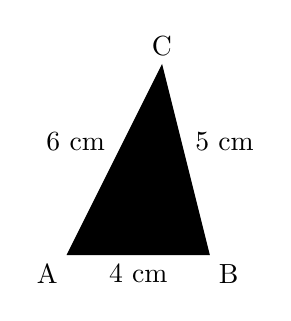
\begin{tikzpicture}[scale=0.6]
            \coordinate[label=below left:A](A)at(0,0);
            \coordinate[label=below right:B](B)at(3,0);
            \coordinate[label=C](C)at(2,4);
            \path(A)--(B)node[midway,below]{4 cm};
            \path(A)--(C)node[midway,above left]{6 cm};
            \path(C)--(B)node[midway,above right]{5 cm};
            \draw[fill=\currentcolor](A)--(B)--(C)--cycle;
        \end{tikzpicture}
    \end{minipage}%
    \begin{minipage}{.4\linewidth}
        $$4+5+6=15$$
        Le périmètre de ABC vaut 15 cm.
    \end{minipage}\hfill\newpage
    \bigpart{Périmètre d'un cercle}
    \proposition{perimetre_d_un_cercle}
    {Exemple :}\vskip10pt
    
\begin{tikzpicture}[baseline=(current bounding box.center)]
        \coordinate(O)at(0,0);
        \coordinate(A)at(30:1.5);
        \coordinate(B)at(210:1.5);
        \draw[fill=\currentcolor](O)circle(1.5);
        \path(B)--(A)node[midway,above,sloped]{9 cm};
        \draw(B)--(A);
    \end{tikzpicture}
    \begin{minipage}[c]{.6\linewidth}
        \begin{align*}
            \text{périmètre}\:&=\:\text{diamètre} \times 3 \\
            &\approx\: 9 \times 3,14 \\
            &\approx\: 28,26
        \end{align*}
        Le périmètre du cercle vaut {\bfseries environ} 28,26~cm.
    \end{minipage}\vskip20pt
    {\bfseries Exemple :}\vskip5pt
    \exported[scale=1,lmargin=30,vmargins=30]%
    <<
        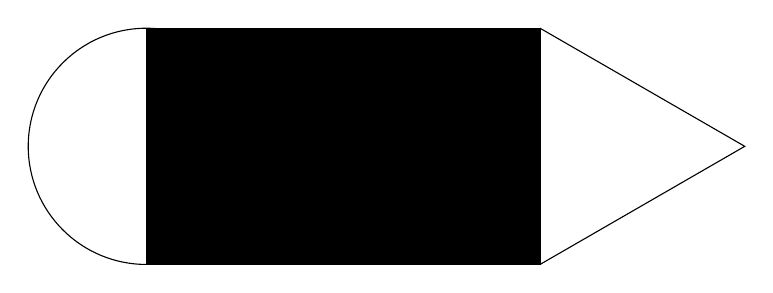
\begin{tikzpicture}
            \coordinate(A)at(0,0);
            \coordinate(B)at(5,3);
            \draw(0,1.5)circle(1.5);
            \draw[draw=\mainbgcolor, fill=\mainbgcolor](A)rectangle(B);
            \draw(A)rectangle(B);
            \draw(5,0)--(7.6,1.5)--(B);
        \end{tikzpicture}
    >>
\end{document}